
We want to develop the calculus necessary to discuss functions
of many variables.   We shall start with functions
$f(x,y)$ of two independent
variables and functions $f(x,y,z)$ of three independent
variables.   However, in general, we need to consider functions
$f(x_1, x_2, \dots, x_n)$ of any number 
of independent variables.   Recall, $\R^n$ stands
for the set of all $n$-tuples $(x_1,x_2,\dots,x_n)$
with real entries $x_i$.  We shall use the old fashioned term \emph{locus}\index{locus}
to denote the set of all points satisfying some equation or condition.

\section{Graphing in Many Variables}

We shall encounter equations involving two, three, or more variables.
As you know, an equation of the form
\[
     f(x,y) = c
\]
may be viewed as defining a curve in the plane.  For example,
$ax + by = c$ defines a line in $\R^2$, while $x^2 + y^2 = r^2$
defines a circle of radius $r$ centered at the origin.
Similarly, an equation involving three variables
\[
   f(x,y,z) = c
\]
may be thought of as defining a \emph{surface} in space.
We saw previously that the locus in $\R^3$ of a linear equation
\[
   ax + by + cz = d
\]
(where not all $a, b$, and $c$ are zero) is a plane.   If we
use more complicated equations, we get more complicated surfaces.

\begin{example}
	The equation
	\[
	   x^2 + y^2 + z^2 = r^2
	\]
	may be rewritten $\norm{\vec r} = \sqrt{x^2 + y^2 + z^2} = R$, so it
	asserts that the point with position vector $\vec r$ is at distance
	$r$ from the origin.  Hence, the locus of all such points is a
	\emph{sphere} of radius $r$ centered at the origin.
\end{example}

\begin{example}
	Consider the locus of the equation
	\[
	  x^2 + 2x + y^2 - 4y + z^2 = 20.
	\]
	This is also a sphere, but one not centered at the origin.  To
	see this, \emph{complete the squares} for the terms involving
	$x$ and  $y$.
	\begin{align*}
	    x^2 + 2x + 1 + y^2 -4y + 4 + z^2 &= 10 + 1 + 4 = 25 \\
	    (x + 1)^2 + (y - 2)^2 + z^2 &= 5^2.
	\end{align*}
	This asserts that the point with position vector $\vec r = ( x, y, z )$
	is 5 units from the point $(-1, 2, 0)$, i.e., it lies on a sphere
	of radius 5 centered at $(-1, 2, 0)$.
\end{example}

\begin{example}
	Consider the locus of the equation $z = x^2 + y^2$ (which could
	also be written $x^2 + y^2 - z = 0$).  To see what this looks like,
	we consider its intersection with various planes.   Its intersection
	with the $yz$-plane is obtained by setting $x = 0$ to get
	$z = y^2$.  This is a parabola in the $yz$-plane.  
	Similarly, its intersection with the $xz$-plane is the parabola
	given by $z = x^2$.   To fill in the picture,  consider
	intersections with planes parallel to the $xy$-plane.  Any
	such plane has the equation $z = h$, so the intersection has the equation
	$x^2 + y^2 = h = (\sqrt h)^2$, which you should recognize as a circle
	of radius $\sqrt h$, if $h > 0$.  Note that the circle is
	centered at $(0,0,h)$ on the $z$-axis since it lies in the plane $z = h$.
	If $z = h = 0$, then the circle reduces to a single point, and for 
	$z = h < 0$, there is no locus.
	The surface is ``bowl'' shaped and is called a \emph{circular
	paraboloid}\index{paraboloid}.

	\begin{center}
	\begin{tikzpicture}
	    \begin{axis}[grid=major,view={20}{20},z buffer=sort,
		    %shader=faceted interp,
		    %patch type=biquadratic,
		    colormap/copper
		    %width=12cm,
		    %scale mode=scale uniformly,
		    %zmin=-5,zmax=5,xmin=-10,xmax=10,ymin=-10,ymax=10,
		    %xticklabels={,,}, yticklabels={,,}, zticklabels={,,},
		    %xtick={-10,-5,...,10}, ytick={-10,-5,...,10}
		    ]
		    \addplot3[surf, domain=-4:4, samples=30]{x*x+y*y};
	    \end{axis}
	  \end{tikzpicture}
	\end{center}
\end{example}

Graphing a surface in $\R^3$ by sketching its traces on various
planes is a useful strategy.  In order to be good at it, you need
to know the basics of plane analytic geometry so you can recognize
the resulting curves.  In particular, you should be familiar with
the elementary facts concerning \emph{conic sections}, i.e.,
ellipses, hyperbolas, and parabolas.   Edwards and Penney, 3rd Edition,
Chapter 10 is a good reference for this material.

\begin{example}
	Consider the locus in space of $\displaystyle{\frac{x^2}4 +
	\frac{y^2} 9} = 1$.   Its intersection with a plane $z = h$
	parallel to the $xy$-plane is an ellipse centered on the $z$-axis
	and with semi-minor and semi-major axes  2 and 3, respectively.   The surface
	is a \emph{cylinder} perpendicular to the $xy$-plane with
	elliptical cross sections.
	Note that the locus \emph{in space} is not just the ellipse
	in the $xy$-plane with the same equation.
	
	\begin{center}
	\begin{tikzpicture}
	    \begin{axis}[grid=major,view={20}{20},z buffer=sort,
		    %shader=faceted interp,
		    %patch type=biquadratic,
		    colormap/copper
		    %width=12cm,
		    %scale mode=scale uniformly,
		    %zmin=-5,zmax=5,xmin=-10,xmax=10,ymin=-10,ymax=10,
		    %xticklabels={,,}, yticklabels={,,}, zticklabels={,,},
		    %xtick={-10,-5,...,10}, ytick={-10,-5,...,10}
		    ]
		    \addplot3[surf, 
		    z buffer=sort,samples=20,
			variable=\u, variable y=\v,
			domain=-180:180, y domain=-2:3]
			({2*cos(u)}, {3*sin(u)}, {v});
	    \end{axis}
	  \end{tikzpicture}
	\end{center}
	XXX Figure
\end{example}

\begin{example}
	Consider the locus in space of the equation
	$z = \dfrac 1{x^2 + y^2}$.   Its intersection with the plane $z = h$
	(for $h > 0$) is the circle with equation
	$ x^2 + y^2 = 1/h = (\sqrt{1/h})^2$.   The surface does not intersect
	the $xy$-plane itself ($z = 0$) nor any plane below the $xy$-plane.
	Its intersection with the $xz$-plane ($y = 0$) is the curve
	$z = 1/x^2$, which is asymptotic to the $x$-axis
	and to the positive $z$-axis.  Similarly, for its intersection
	with the $yz$-plane,   the surface flattens out and approaches the
	$xy$-plane as $r = \sqrt{x^2 + y^2} \to \infty$.  It approaches the
	positive $z$-axis as $r \to 0$.


	\begin{center}
	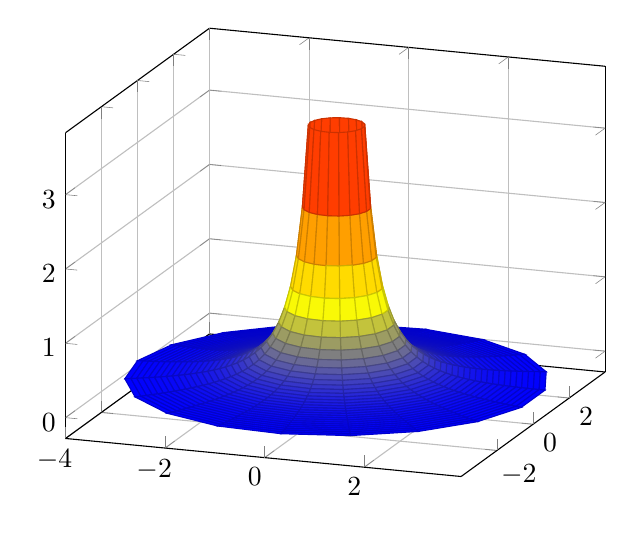
\begin{tikzpicture}
	    \begin{axis}[grid=major,view={20}{20},z buffer=sort,
		    %shader=faceted interp,
		    %patch type=biquadratic,
		    colormap/hot,
		    %width=12cm,
		    %scale mode=scale uniformly,
		    %zmin=-5,zmax=5,xmin=-10,xmax=10,ymin=-10,ymax=10,
		    %xticklabels={,,}, yticklabels={,,}, zticklabels={,,},
		    %xtick={-10,-5,...,10}, ytick={-10,-5,...,10}
		    unbounded coords=jump,
		    restrict z to domain=0:5
		    ]
		    %\addplot3[surf, domain=-4:4, samples=30]{1/(x*x+y*y)};
		    \addplot3[surf, 
		    z buffer=sort,samples=20, samples y=35,
			variable=\u, variable y=\v,
			domain=-180:180, y domain=.2:4]
			({v*cos(u)}, {v*sin(u)}, {1/(v*v)});
	    \end{axis}
	  \end{tikzpicture}
	\end{center}
\end{example}

\begin{example}
	Consider the locus in space of the equation $yz = 1$.   Its intersection
	with a plane parallel to the $yz$-plane ($x = d$) is a hyperbola
	asymptotic to the $y$ and $z$ axes.  The surface is perpendicular
	to the $yz$-plane.  Such a surface is also called a \emph{cylinder},
	although it doesn't close upon itself as the elliptical cylinder considered
	above.
\end{example}

\begin{example}
	Consider the locus of the equation $x^2 + z^2 = y^2 - 1$.  For
	each plane parallel to the $xz$-plane ($y = c$), the intersection
	is a circle $x^2 + z^2 = c^2 - 1 = \left(\sqrt{c^2 - 1}\right)^2$ centered
	on the $y$-axis, at least of $c^2 > 1$.  For $y = c = \pm 1$,
	the locus is a point, and for $-1 < y = c < 1$, the locus is
	empty.   In addition, the intersection of the surface with the
	$xy$-plane ($z = 0$) is the hyperbola with equation $x^2 - y^2
	 = -1$, and similarly for its intersection with the $yz$-plane.
	The surface comes in two pieces which open up as ``bowls'' centered
	on the positive and negative $y$-axes.   The surface is called
	a \emph{hyperboloid of 2 sheets}.    
	
	\begin{center}
	\begin{tikzpicture}
	    \begin{axis}[grid=major,view={60}{40},z buffer=sort,
		    %shader=faceted interp,
		    %patch type=biquadratic,
		    colormap/copper,
		    %width=12cm,
		    %scale mode=scale uniformly,
		    %zmin=-5,zmax=5,xmin=-10,xmax=10,ymin=-10,ymax=10,
		    %xticklabels={,,}, yticklabels={,,}, zticklabels={,,},
		    %xtick={-10,-5,...,10}, ytick={-10,-5,...,10}
		    unbounded coords=jump,
		    ]
		    %\addplot3[surf, domain=-4:4, samples=30]{1/(x*x+y*y)};
		    \addplot3[surf, 
		    z buffer=sort,samples=40, samples y=15,
			variable=\u, variable y=\v,
			domain=-180:180, y domain=0:4]
			({v*cos(u)}, {sqrt(v*v+1)}, {v*sin(u)});
		    \addplot3[surf, 
		    z buffer=sort,samples=40, samples y=15,
			variable=\u, variable y=\v,
			domain=-180:180, y domain=0:4]
			({v*cos(u)}, {-sqrt(v*v+1)}, {v*sin(u)});
	    \end{axis}
	  \end{tikzpicture}
	\end{center}
\end{example}

\subsection{Graphing Functions}
For a scalar function $f$ of one independent variable, 
the \emph{graph of the function} is the set of
\index{graph of a function}
all points in $\R^2$  of the form  $(x, f(x))$
for $x$ in the domain of the function.   (The domain of a function
is the set of values of the independent variable for which the
\index{domain of a function}
function is defined).  In other words, it is the locus of the
equation $y = f(x)$.  It is generally a curve in the plane.

We can define a similar notion for a scalar function $f$ of two
independent variables.  The graph is the
set of points in $\R^3$  of the form $(x, y, f(x,y))$
for $(x,y)$, a point in the domain of the function.  In other words,
it is the locus of the equation $z = f(x,y)$, and it is generally
a surface in space.
The graph of a function is often useful in understanding the
function.

We have already encountered several examples of graphs of functions.
For example, the locus of $z = x^2 + y^2$ is the graph of the
function $f$ defined by $f(x,y) = x^2 +y^2$.   Similarly, the locus
of $z = 1/(x^2 + y^2)$ is the graph of the function $f$ defined by
$f(x,y) = 1/(x^2 + y^2)$ for $(x,y) \not= (0,0)$. 
  Note that in the first case there does not need to be a restriction on the domain of the function, but in the second
case $(0,0)$ was omitted.  

In some of the other examples, the locus
of the equation cannot be considered the graph of a function.
For example, the equation $x^2 + y^2 + z^2 = R^2$ cannot be solved
uniquely for $z$ in terms of $(x,y)$.  Indeed, we have
$z = \pm\sqrt{R^2 - x^2 - y^2}$, so that two possible functions
are suggested.  $z = f_1(x,y) = \sqrt{R^2 - x^2 - y^2}$ 
defines a function with graph
the \emph{top hemisphere}, while $z = f_2(x,y)
= - \sqrt{R^2 - x^2 - y^2}$ yields the lower hemisphere.  (Note that
for either of the functions, the relevant domain is the set of
points on or inside the circle $x^2 + y^2 = R^2$.  For points outside
that circle, the expression inside the square root is negative, and
since we are only talking about functions assuming real values,
such points must be excluded).

\begin{example}
	Let $f(x,y) = xy$ for all $(x,y)$ in $\R^2$.    The graph is the
	locus of the equation $z = xy$.  We can sketch it by considering
	traces on various planes.  Its intersection with a plane parallel
	to the $xy$-plane ($z =$ constant) is a hyperbola asymptotic to
	lines parallel to the $x$ and $y$ axes.   For $z > 0$, the hyperbola
	is in the first and third quadrants of the plane, but for
	$z < 0$, it is in the second and fourth quadrants.  For $z = 0$,
	the equation is $xy = 0$ with locus consisting of the $x$-axis
	($y = 0$) and the $y$-axis ($x = 0$).   Thus, the graph intersects
	the $xy$-plane in two straight lines.  The surface is generally
	shaped like an ``infinite saddle.''  It is called a {\it hyperbolic
	paraboloid}.  It is clear where the term ``hyperbolic'' comes from.
	Can you see any parabolas?  (Hint: Try planes perpendicular to
	the $xy$-plane with equations of the form  $y = mx$).

	%\begin{center}
	%\begin{tikzpicture}
	%    \begin{axis}[grid=major,view={20}{20},z buffer=sort,
	%	    colormap/copper,
	%	    unbounded coords=jump,
	%	    restrict y to domain=-6:6
	%	    ]
	%	    \addplot3[surf, domain=-4:4, samples=50]({x}, {1/x}, {1});
	%	    \addplot3[surf, domain=-4:4, samples=50]({x}, {2/x}, {2});
	%	    \addplot3[surf, domain=-4:4, samples=50]({x}, {3/x}, {3});
	%	    \addplot3[surf, domain=-4:4, samples=50]({x}, {-1/x}, {-1});
	%	    \addplot3[surf, domain=-4:4, samples=50]({x}, {-2/x}, {-2});
	%	    \addplot3[surf, domain=-4:4, samples=50]({x}, {-3/x}, {-3});
	%    \end{axis}
	%  \end{tikzpicture}
	%\end{center}
	
	\begin{center}
	\begin{tikzpicture}
	    \begin{axis}[grid=major,view={20}{20},z buffer=sort,
		    colormap/copper
		    ]
		    \addplot3[surf, domain=-4:4, samples=30]{x*y};
	    \end{axis}
	  \end{tikzpicture}
	\end{center}
\end{example}

\begin{example}
	 Let $f(x,y) = x/y$ for $y \not= 0$.  Thus, the domain of this
	function consists of all points $(x,y)$ not on the $x$-axis
	($y = 0$).
	The trace in the plane $y = c, c \not= 0$ is the line $z = (1/c)x$
	with slope $1/c$.   Similarly, the trace in the plane $z = c, c \not=0$
	is the line $y = (1/c)x$.  Finally, the trace in the plane $x = c$,
	is the hyperbola $z = c/x$.  Even with this information you will have
	some trouble visualizing the graph.   However, the equation
	$z = x/y$ can be rewritten $yz = x$.   By permuting the variables,
	you should see that the locus of $yz = x$
	 is similar to the  saddle-shaped surface
	we just described but oriented differently in space.  However,
	 the saddle
	is not quite the graph of the function since it  contains the 
	 $z$-axis ($y = x = 0$) but the graph of the function does not.
	In general, the graph of a function, since it consists of points
	of the form $(x,y,f(x,y))$, cannot contain points with the same
	values for $x$ and $y$ but different values for $z$.  In other words,
	any line parallel to the $z$-axis can intersect such a graph at most
	once. 
\end{example}

Sketching graphs of functions, or more generally loci of equations
in $x, y$, and $z$, is not easy.   One approach drawn from the
study of topography is to interpret the equation $z = f(x,y)$ as
giving the \emph{elevation} of the surface, viewed as a hilly
terrain, above a reference plane.  (Negative elevation
 $f(x,y)$ is
interpreted to mean that the surface dips below the reference plane.)
For each possible elevation $c$,
 the intersection of the plane $z = c$ with the graph
yields a curve $f(x,y) = c$.  This curve is called a \emph{level curve}, 
and we draw a 2-dimensional map of the graph by sketching
\index{level curve}
the level curves and labeling each by the appropriate elevation
$c$.  Of course, there are generally infinitely many level curves
since there are infinitely many possible values of $z$, but we
select some subset to help us understand the topography of the
surface.

XXX Figure

\begin{example}
	The level curves of the surface $z = xy$ have equations
	$xy = c$ for various $c$.  They form 
	a family of hyperbolas, each with two branches.  For $c > 0$,
	these hyperbolas fill the first and third quadrants, and for
	$c < 0$ they fill the second and fourth quadrants.  For $c  = 0$
	the $x$ and $y$ axes together constitute the level ``curve.''
	See the diagram.

	You can see that the region around the origin $(0,0)$ is like a
	``mountain pass'' with the topography rising in the first and
	third quadrants and dropping off in the second and fourth quadrants.
	In general, a point where the graph behaves this way is called
	a \emph{saddle point}.   Saddle points indicate the added complexity
	which can arise when one goes from functions of one variable to
	functions of two or more variables.  At such points, the function
	can be considered as having a maximum  or
	 a minimum depending on where you
	look.
\end{example}

\subsection{Quadric Surfaces}
One important class of surfaces are those defined by quad\-rat\-ic
equations.  These are analogs in three dimensions of
conics in two dimensions.  They are called \emph{quadric surfaces}.  
We describe here \emph{some} of the possibilities.
You can verify the pictures by using the methods described above.
\index{quadric surface}

Consider first equations of the form
\[
   \pm \frac{x^2}{a^2} 
   \pm \frac{y^2}{b^2} 
   \pm \frac{z^2}{c^2} = 1
\]

If all the signs are positive, the surface is called an {\it 
ellipsoid}.
\index{ellipsoid}
Planes perpendicular to one of the coordinate axes intersect it
in ellipses (if they intersect at all).   However, at the extremes
these ellipses degenerate into the points $(\pm a, 0, 0),
(0,\pm b, 0)$, and $(0,0,\pm c)$.

XXX Figure

If exactly one of the signs are negative, the surface is called a
\emph{hyperboloid of one sheet}.   It is centered on one axis
\index{hyperboloid of one sheet}
(the one associated with the negative coefficient in the equation)
and it opens up in both positive and negative directions along
that axis.  Its intersection with planes perpendicular to that
axis are ellipses.   Its intersections with planes perpendicular to
the other axes are hyperbolas.


If exactly two of the signs are negative, the surface is called
a \emph{hyperboloid of two sheets}.   It is centered on one
\index{hyperboloid of two sheets}
axis (associated with the positive coefficient).  For example,
suppose the equation is
\[
  -\frac{x^2}{a^2}
  +\frac{y^2}{b^2}
  -\frac{z^2}{c^2} = 1.
\]
For $y < -b$ or $y > b$, the graph intersects a plane perpendicular
to the $y$-axis in an ellipse.  For $y = \pm b$, the intersection
is the point $(0,\pm b, 0)$.  (These two points are called vertices
of the surface.)  For $-b < y < b$, there is no intersection with
a plane perpendicular to the $y$-axis.


The above surfaces are called \emph{central quadrics}.
\index{central quadric}
Note that for the hyperboloids, with equations in standard form as
above, the number of sheets is the same as
the number of minus signs.

Consider next equations of the form
\[
   z = \pm \frac{x^2}{a^2} \pm \frac{y^2}{b^2}
\]
(or similar equations obtained by permuting $x, y$ and $z$).

If both signs are the same, the surface is called an {\it elliptic
paraboloid}.   If both signs are positive, it is centered on the
\index{elliptic paraboloid}
\index{paraboloid, elliptic}
positive $z$-axis and its intersections with planes perpendicular to
the positive $z$-axis are a family of similar ellipses which increase
in size as $z$ increases.   If both signs are negative, the situation
is similar, but the surface lies below the $x,y$ plane.


If the signs are different, the surface is called a {\it
hyperbolic paraboloid}.  Its intersection with planes perpendicular
to the $z$-axis are hyperbolas asymptotic to the lines in
those planes parallel to the lines $x/a = \pm y/b$.   Its intersection
with the $xy$-plane is just those two lines.  The surface has
a saddle point at the origin.
\index{hyperbolic paraboloid}
\index{paraboloid, hyperbolic}
\index{saddle}


The locus of the equation $z = cxy, c\not= 0$ is also a hyperbolic
paraboloid, but rotated so it intersects the $xy$-plane in the
$x$ and $y$ axes. 

XXX Figure

Finally, we should note that many so called ``degenerate conics''
are loci of quadratic equations.   For example, consider
\[
    \frac{x^2}{a^2} + \frac{y^2}{b^2} - \frac{z^2}{c^2} = 0
\]
which may be solved to obtain
\[
   z = \pm c\sqrt{\frac{x^2}{a^2} + \frac{y^2}{b^2}}. 
\]

The locus is a double cone with elliptical cross sections and
vertex at the origin.  

\subsection{Generalizations}
In general, we will want to study functions of any number of independent
variables.   For example, we may define the graph of a scalar valued
function $f$ of three independent variables to be the set of all points
in $\R^4$ of the form $(x,y,z,f(x,y,z))$.   Such an object
should be considered a three dimensional subset of $\R^4$, and it is
certainly not easy to visualize.  It is more useful to consider the
analogs of level curves for such functions.  Namely, for each
possible value $c$ attained by the function, we may consider the
locus in $\R^3$ of the equation $f(x,y,z) = c$.  This is generally
a surface called a \emph{level surface} for the function. 
\index{level surface}

\begin{example}
For $f(x, y, z) = x^2 + y^2 + z^2$, the level surfaces are
concentric spheres centered at the origin if $c > 0$.   For
$c = 0$ the level `surface' is not really a surface at all; it
just consists of the point at the origin.   (What if $c < 0$?) 

For $f(x,y,z) = x^2 + y^2 - z^2$, the level surfaces are either
hyperboloids of one sheet if $c > 0$ or hyperboloids of two sheets
if $c < 0$.  (What if $c = 0$?)
\end{example}

For functions of four or more variables, geometric interpretations
are even harder to come by.  If $f(x_1,x_2,\dots,x_n)$ denotes
a function of $n$ variables, the locus in $\R^n$  of the
equation $f(x_1,x_2,\dots,x_n) = c$ is called a level set,
but one doesn't ordinarily try to visualize it geometrically.  

Instead of talking about many independent variables, it is useful
to think instead of a single independent variable which is a 
\emph{vector}, i.e., an element of $\R^n$ for some $n$.   In the
case  $n = 2, 3$, we usually write $\vec r = ( x,y )$ or
$\vec r = ( x,y,z )$ so $f(x,y)$ or $f(x,y,z)$ would be written 
simply $f(\vec r)$.  If $n > 3$, then one often denotes the
variables $x_1, x_2, \dots, x_n$ and denotes the vector
(i.e., element of $\R^n$) by $\vec x = (x_1,x_2, \dots, x_n)$.
Then $f(x_1,x_2, \dots, x_n)$ becomes simply  $f(\vec x)$.
The case of a function of a single real variable can be subsumed
in this formalism by allowing the case $n =1$.  That is,
we consider a scalar $x$ to be just a vector of dimension 1,
i.e., an element of $\R^1$.

When we talked about kinematics, we considered  \emph{vector valued}
functions $\vec r(t)$ of a single independent variable.    Thus we see
that it makes sense to consider in general functions of a vector
variable which can also assume vector values.   We indicate this
by the notation $f:\R^n \to \R^m$.   That shall mean that the domain
of the function $f$ is a subset of $\R^n$ while the set of values is
a subset of $\R^m$.    Thus, $n = m = 1$ would yield a scalar
function of one variable, $n = 2, m = 1$ a scalar function of two
variables, and $n = 1, m = 3$ a vector valued function of one scalar
variable.   We shall have occasion to consider several other special
cases in detail.

There is one slightly non-standard aspect to the above notation.
In ordinary usage in mathematics,
``$f:\R^n \to \R^m$'' means that $\R^n$ is the entire domain of the
function $f$, whereas we are taking it to mean that the domain is some
subset.    We do this mostly to save writing since usually the
domain will be almost all of $\R^n$  or at least some significant
chunk of it.  What we want to make clear by the notation is the
dimensionality of both the independent and dependent variables.

\begin{exercises}
You are encouraged to make use of the available computer software
(e.g., Maple, Mathematica, etc.) to help you picture the graphs
in the following problems.


\begin{enumerate}
	\item   State the largest possible domain for the function 
	\begin{enumerate}
		\item $f(x,y) =  e^{ x^2-y^2}$ 
		\item $f(x,y) = \ln (y^2-x^2-2)$ 
		\item $f(x,y) = \dfrac {x^2-y^2}{x-y}$ 
		\item $f(x,y,z) = \dfrac {1}{xyz}$ 
		\item $f(x,y,z) = \dfrac {1}{\sqrt {z^2-x^2-y^2}}$ 
	\end{enumerate}

	\item   Describe the graph of the function described by 
	\begin{enumerate}
		\item $f(x,y) = 5$ 
		\item $f(x,y) = 2x - y$ 
		\item $f(x,y) = 1-x^2-y^2$ 
		\item $f(x,y) = 4 - \sqrt {x^2+y^2}$ 
		\item $f(x,y) = \sqrt {24 - 4x^2 - 6y^2}$ 
	\end{enumerate}

	\item   Sketch selected level curves for the functions given by
	\begin{enumerate}
		\item $f(x,y) = x+y$
		\item $f(x,y) = x^2 + 9y^2$
		\item $f(x,y) = x - y^2$
		\item $f(x,y) = x - y^3$
		\item $f(x,y) = x^2 + y^2 + 4x + 2y +9$
	\end{enumerate}

	\item   Describe selected level surfaces for the functions
	given by 
	\begin{enumerate}
		\item $f(x,y,z) = x^2 + y^2 - z$ 
		\item $f(x,y,z) = x^2 + y^2 + z^2 + 2x - 2y + 4z$ 
		\item $f(x,y,z) = z^2 - x^2 - y^2$ 
	\end{enumerate}

	\item   Describe the quadric surfaces which are loci in $\R^3$
	of the following equations. 
	\begin{enumerate}
		\item $x^2 + y^2 = 16$ 
		\item $z^2 = 49x^2 + y^2$ 
		\item $z= 25 - x^2 - y^2$ 
		\item $x=4y^2-z^2$ 
		\item $4x^2 + y^2 + 9z^2 = 36$ 
		\item $x^2 + y^2 - 4z^2 = 4$ 
		\item $9x^2 + 4y^2 -z^2 = 36$ 
		\item $9x^2 - 4y^2 - z^2 = 36$
	\end{enumerate}

	\item   Describe the traces of the following functions in the given planes
	\begin{enumerate}
		\item $z=xy$, in horizontal planes  $z = c$ 
		\item $z=x^2+9y^2$ in vertical planes $x = c$ or $y = c$ 
		\item $z=x^2+9y^2$ in horizontal planes  $z = c$
	\end{enumerate}

	\item   Describe the intersection of the cone $x^2 + y^2 = z^2$ with
	the plane $z = x + 1$.  

	\item   Let $\vec f:\R^2 \to \R^2$.  
	\begin{enumerate}
		\item Try to invent a definition of `graph' for such a function.   For
		    what $n$ would it be a subset of $\R^n$? 
		\item Try to invent a definition of `level set' for such a function.
		    For what $n$ would it be a subset of $\R^n$?
	\end{enumerate}

\end{enumerate}
\end{exercises}

\section{Rates of Change and the Directional Derivative}
	
For a function $f:\R\to\R$ of one variable, we have the idea of
the \emph{rate of change} of $f$.  We might ask, ``rate of change with
respect to what?''  For a function of one variable, this question has an obvious
answer---the rate of change with respect to the only thing that varies!
If $g:\R^n\to\R$ is a multi-variable function, the question of ``what is the rate of change
of $g$?'' has a less obvious answer.  After all, there are multiple variables and
infinitely many directions in the domain.

Consider the function $g:\R^2\to\R$ where $g(x,y)=(x-2)^2+y^2$.  Let $\vec u$ be a unit
vector.  Now, starting at $(0,0)$, we might ask approximately how much $g$ changes
when we move $\alpha$ units away from $(0,0)$ in the direction $\vec u$.

XXX Figure

Since $\vec u$ is a unit vector, the displacement in the domain is $\alpha\vec u$, and so the
exact change in $g$ from $\vec 0$ to $\alpha\vec u$ is $g(\alpha\vec u)-g(\vec 0)$.  The approximate
\emph{rate} of change\index{rate of change} is then $\frac{g(\alpha\vec u)-g(\vec 0)}{\alpha}$.  Taking
a limit as $\alpha\to 0$ will give us an instantaneous rate of change---one worth name.

\begin{definition}[Rate of change with respect to distance]
	For a function $f:\R^n\to\R$, the \emph{rate of change with respect to distance} of $f$
	in the direction $\vec v$ at the point $\vec a$ is
	\[
		\lim_{h\to 0^+}\frac{f(\vec a+h\vec v)-f(\vec a)}{\norm{h\vec v}}.
	\]
\end{definition}

We must divide by $\norm{h\vec v}$ in the definition of rate of change with respect to distance
because $\norm{h\vec v}$ is exactly how far we've displaced.  Of course, if we were forward-thinking
enough to pick $\vec v$ to be a unit vector, then $\norm{h\vec v}=\abs{h}$.

We can think of the rate of change with respect to distance in another way.  Suppose that $f:\R^n\to \R$
and that $\vec p:\R\to\R^n$ is the arc-length parameterization of the with direction
vector $\vec v$ and where $\vec p(0)=\vec a$.  Then $f\circ \vec p:\R\to\R$ is a single-variable
function and the rate of change of $\vec f$ at $\vec a$ in the direction $\vec v$ is just $(f\circ\vec p)'(0)$.
Think for a moment about why this is.

The rate of change of a function with respect to distance is, in some sense, the most natural
notion of ``rate of change'' for a multivariable function.  (If you're handed a function, what
would you measure the rate of change against if not distance?)  However, it turns out not
to be the most useful notion of rate of change.  For that, we introduce the 
\emph{directional derivative}\index{directional derivative}.

\begin{definition}[Directional Derivative]
	For a function $f:\R^n\to\R$, the \emph{directional derivative} of $f$ at the point $\vec a$
	in the direction $\vec v$ is
	\[
		D_{\vec a}f(\vec v) = \lim_{h\to0}\frac{f(\vec a+h\vec v)-f(\vec a)}{h}.
	\]
\end{definition}

The directional derivative $D_{\vec a}f(\vec v)$ corresponds to the rate of change of $f$ at the point $\vec a$
if you moved in the direction of $\vec v$ with speed $\norm{\vec v}$.  This seems 
like a less intuitive notion than the rate of change with respect to distance, but its virtues will
soon become clear\footnote{ For starters, $D_{\vec a}f$ is \emph{linear}.  Namely, if $f$ is differentiable,
then $D_{\vec a}f(\vec u+\vec v)=D_{\vec a}f(\vec u)+D_{\vec a}f(\vec v)$.  The same cannot
be said for the rate of change with respect to distance.}.

\begin{example}
	Let $f:\R^2\to\R$ be given by $f(x,y)=(x-2)^2-y^2$.  Compute $D_{\vec 0}f(1,2)$.

	Since we have no further theory to lean on, we must use the definition of the directional
	derivative directly.

	\begin{align*}
		D_{\vec 0}f(1,2) &= \lim_{h\to0}\frac{f(\vec 0+h(1,2))-f(\vec 0)}{h}
		=\lim_{h\to0}\frac{((h-2)^2-(2h)^2)-4}{h}\\
		&=\lim_{h\to0}\frac{(-3h^2-4h+4)-4}{h}=-4.
	\end{align*}
\end{example}

The directional derivative can be used to approximate a function.  Recall that if $g:\R\to\R$ is
a differentiable function of one variable, then
\[
	g(a+h)\approx f(a) + hg'(a).
\]
Similarly, for $f:\R^2\to\R$ we have\footnote{ Assuming $f$ has directional derivatives, of course.}
\begin{equation}
	\label{EQDIRDERIVAPPROX}
	f(\vec a+h\vec v)\approx f(\vec a)+hD_{\vec a}f(\vec v).
\end{equation}

The similarity in these two formulas is one reason
why directional derivatives are more useful than rates of change with respect to distance\footnote{
	If we think about vectors in $\R^1$, the number $1$ is actually a vector.  Therefore,
	for $g:\R\to\R$, we have $g'(1)=D_{a}g(1)$.  Try writing out the limit expression.  It's the same
	as the usual definition of derivative!
	}.

\begin{exercise}
	Create the analogous equation to Equation \eqref{EQDIRDERIVAPPROX} but approximate
	$f(\vec a+h\vec v)$ using the rate of change with respect to distance instead of the
	directional derivative.
\end{exercise}


\subsection{Partial Derivatives}
There are some particularly common directional derivatives.  Namely, those in the directions
of the standard basis.  Let $f:\R^2\to\R$ and let $\vec a=(a_x,a_y)$.  Now,
\begin{align*}
	D_{\vec a}f(\xhat) &= \lim_{h\to0}\frac{f(\vec a+h\xhat)-f(\vec a)}{h}
	=\lim_{h\to0}\frac{f(a_x+h, a_y)-f(a_x,a_y)}{h}.
\end{align*}

This limit looks quite similar to a one-dimensional derivative.  However, $f$ does not
have a one-dimensional domain.  Accordingly we call $D_{\vec a}f(\xhat)$ a 
\emph{partial derivative}\index{partial derivative} and we have a special notation for it.

\begin{definition}
	For a function $f:\R^n\to\R$, let $x_i$ denote the $i$th input variable.
	The \emph{partial derivative} of $f$ at $\vec a=(a_1,\ldots,a_n)$ with respect to $x_i$ is 
	notated $\frac{\partial f}{\partial x_i}(\vec a)$ and is defined to be
	\[
		\frac{\partial f}{\partial x_i}(\vec a) = 
		\lim_{h\to0}\frac{f(a_1,\ldots,a_{i-1},a_i+h,a_{i+1},\ldots,a_n)-f(\vec a)}{h}.
	\]
\end{definition}
Sometimes we'll write $\frac{\partial f}{\partial x_i}$, omitting the point where the partial
derivative is taken, if we want to save space, or if we want to view a partial derivative as a function
of where it is taken.  For functions whose domains are $\R^2$ or $\R^3$, we often use $x,y,z$ 
instead of $x_1,x_2,x_3$ to denote
the first, second, or third variable.  It is not important how you write your variable as long
as it is clear to you and your reader which variable is changing.

\subsection{Tangent Vectors to Surfaces}
When we had a curve $\mathcal S$ parameterized by $\vec p:\R\to\mathcal S$,
we could find tangent vectors to $\mathcal S$ by computing the velocity vectors of $\vec p$.
In particular, $\vec p\,'(t_0)$ is a tangent vector to $\mathcal S$ at the point $\vec p(y_0)$.
We will find tangent vectors to surfaces in a similar way---by parameterizing a path on the surface.

Suppose $f:\R^2\to \R$ is a function and let $\mathcal S$ be the surface given by $z=f(x,y)$.  Formally,
\[
	\mathcal S=\Set*{\mat{x\\y\\z}\given z=f(x,y)}.
\]
Since $\mathcal S$ is the graph of a function whose domain is $\R^2$ we have a natural parameterization
of $\mathcal S$ coming from $f$.  That is,
\[
	\vec p:\R^2\to\mathcal S\qquad\text{where}\qquad \vec p(x,y)=\matc{x\\y\\f(x,y)}
\]
is a parameterization of $\mathcal S$.

Let $\vec a=(a_x,a_y,f(a_x,a_y))\in\mathcal S$ and consider the function $\vec r_x:\R\to\R^2$
given by $\vec r_x(t) = (a_x+t,a_y)$.  The function $\vec r_x$ starts at the point $(a_x,a_y)$
in the $xy$-plane and moves parallel to the $x$-axis with speed one.  Since we have parameterized
$\mathcal S$ by the $xy$-plane, by composing $\vec p$ and $\vec r_x$, we will get a parameterization
of a curve on $\mathcal S$.  That is, $\vec c=\vec p\circ \vec r_x$ parameterizes the curve
on the surface $\mathcal S$ that when viewed from above looks like the line $y=a_y$.

XXX Figure

Further, $\vec c(0)=(a_x,a_y,f(a_x,a_y))=\vec a$.  Thus, if we want a tangent
vector to $\mathcal S$ at $\vec a$, all we need to do is compute $\vec c\,'(0)$.

Computing,
\[
	\vec c\,'(0)=(\vec p\circ \vec r_x)'(0)=
	\left(\matc{a_x+t\\a_y\\f(a_x+t,a_y)}'\text{ at $t=0$ } \right)
	= \matc{1\\0\\\frac{\partial f}{\partial x}(a_x,a_y)}.
\]

Of course, this was just one choice of a curve along $\mathcal S$.  We could
have just as easily used $\vec p\circ \vec r_y$ where $\vec r_y(t)=(a_x,a_y+t)$
as a parameterization of a curve.  We could have parameterized paths
that weren't parallel to the $x$ or $y$ axes.  For instance
$\vec p\circ \vec r_{d}$ where $\vec r_{d}(t) = (a_x+td_x, a_y+td_y)$
for non-zero constants $d_x,d_y$.

\begin{example}
	Find at least three tangent vectors at the point $\vec a=(1,2,12)$
	to the surface $\mathcal S$ defined by $z=f(x,y)$ where $f(x,y)=(x-3)^2+y^3$.

	Let $\vec r_a(t) = (1+t,2)$, $\vec r_b(t)=(1,2+t)$, and $\vec r_c(t)=
	(1+t,2+t)$.  Further, let $\vec p:\R^2\to\R^3$ be defined by $\vec p(x,y)=
	(x,y,f(x,y))$.  Since $\vec p$ is a parameterization of $\mathcal S$,
	$\vec p\circ \vec r_a$, $\vec p\circ \vec r_b$, 
	and $\vec p\circ \vec r_c$ all parameterize paths in $\mathcal S$.  Further,
	\[\vec p\circ \vec r_a(0)=\vec p\circ \vec r_b(0)=\vec p\circ \vec r_c(0)=\vec a,\]
	so the velocity vectors at $t=0$ of these parameterizations will give 
	tangent vectors to $\mathcal S$ at $\vec a$.
	
	Computing, we see
	\[
	(\vec p\circ \vec r_a)'(0)
	= \matc{1\\0\\\frac{\partial f}{\partial x}(1,2)} = \mat{1\\0\\-4},
	\]
	\[
	(\vec p\circ \vec r_b)'(0)
	= \matc{0\\1\\\frac{\partial f}{\partial y}(1,2)} = \mat{0\\1\\12},
	\]
	and
	\[
	(\vec p\circ \vec r_c)'(0)
	= \matc{1\\1\\ D_{(1,2)}f(1,1)} = \mat{1\\1\\8}
	\]
	are all tangent vectors to $\mathcal S$ at $\vec a$.
\end{example}



\begin{exercises}
\end{exercises}

\section{Tangent Planes and Differentiability}

Suppose $f:\R^2\to\R$ is a function and consider the surface $\mathcal S\subseteq \R^3$
given by the equation $z=f(x,y)$.  If $f$ is a ``nice'' function, like a polynomial, 
the surface $\mathcal S$ will be smooth.  Visually, at each point on $\mathcal S$ we
could imagine a tangent plane---the analog of a tangent line to a curve.

XXX Figure

More formally, fix a point $\vec a\in\mathcal S$ and consider the set $\mathcal P$
of all tangent vectors to $\mathcal S$ at $\vec a$.  If $\mathcal S$ is a smooth
surface, these tangent vectors will lie in a single plane.  In other words,
$\mathcal P$ is a plane, and in this case we call it the 
\emph{tangent plane}\index{tangent plane}
to $\mathcal S$ at $\vec a$.  (Fantastically, if $\mathcal P$ is a plane,
it can be fully described by the point $\vec a$ and \emph{two} non-parallel
tangent vectors.  We'll make use of this idea later.)

XXX Figure

Tangent planes to surfaces, like tangent lines to curves, have
the property that they are a very good approximation to a surface
at their point of tangency.  We will leverage this idea to 
define what it means to be differentiable for a multivariable function.

\subsection{Directional Derivatives and Planes}

A plane $\mathcal P$ is a \emph{set} and is distinct from any equations
or parameterizations.  However, if $\mathcal P\subseteq \R^3$ is not a vertical
plane (i.e., one for which $\zhat$ is a direction vector), then it can be represented
uniquely by an equation of the form $z=\alpha x+\beta y+c$.  In other words,
a non-vertical plane in $\R^3$ is the graph of a function $f:\R^2\to\R$
which takes the form $f(x,y)=\alpha x+\beta y+c$.  Functions of this form
are known as \emph{affine functions}\index{affine function}, and they
often show up in the context of \emph{linear approximations}\index{linear approximations}\footnote{
	In many contexts in calculus, the term ``linear approximation'' is used
	where ``affine approximation'' would be more accurate.  Sometimes, though,
	it's easiest not to fight the tide of established culture.}.

\begin{definition}[Affine Function]
	A function $f:\R^n\to\R$ is an \emph{affine function} if it can
	be expressed as
	\[
		f(x_1,x_2,\ldots,x_n) = \alpha_1x_1+\alpha_2x_2+\cdots+\alpha_nx_n +c
	\]
	for some $\alpha_1,\ldots,\alpha_n,c\in\R$.  Equivalently, $f:\R^n\to\R$ is
	an affine function if it can be expressed as
	\[
		f(\vec x)=\vec \alpha \cdot \vec x+c
	\]
	for some $\vec\alpha\in\R^n$ and $c\in \R$.
\end{definition}


Directional derivatives of affine functions take a particularly nice form.
Let $f:\R^2\to\R$ be an affine function.
That is, $f(x,y)=\alpha x+\beta y+c$ for some $\alpha,\beta,c\in\R$. 
Let $\vec a=(a_x,a_y)$ and $\vec v=(v_x,v_y)$.  Now,

\begin{align*}
	D_{\vec a}f(\vec v) &= \lim_{h\to0}\frac{f(\vec a+h\vec v)-f(\vec a)}{h}
	=\lim_{h\to0}\frac{f(a_x+hv_x, a_y+hv_y)-f(a_x,a_y)}{h}\\
	&=\lim_{h\to0}\frac{\alpha(a_x+hv_x)+\beta( a_y+hv_y)+c-(\alpha a_x+\beta a_y+c)}{h}\\
	&=\lim_{h\to0}\frac{\alpha hv_x+\beta hv_y}{h} = \alpha v_x+\beta v_y\\
	&=\mat{\alpha\\\beta}\cdot \vec v.
\end{align*}

We have written a formula for the directional derivative of $f$ in an arbitrary direction!  There's more.
\[
	\alpha = \mat{\alpha\\\beta}\cdot \xhat = \frac{\partial f}{\partial x}(\vec a)
	\qquad\text{ and }\qquad
	\beta = \mat{\alpha\\\beta}\cdot \yhat = \frac{\partial f}{\partial y}(\vec a)
\]
and so
\[
	D_{\vec a}f(\vec v) = \mat{\tfrac{\partial f}{\partial x}(\vec a)\\[3pt]\tfrac{\partial f}{\partial y}(\vec a)}
	\cdot \vec v.
\]
The vector $\mat{\tfrac{\partial f}{\partial x}(\vec a)\\[3pt]\tfrac{\partial f}{\partial y}(\vec a)}$ comes up often.
It is called the \emph{gradient}\index{gradient}.

\begin{definition}[Gradient]
	For a function $f:\R^n\to\R$, the \emph{gradient} of $f$ at the point $a$ is
	written $\nabla f(\vec a)$ and is defined to be the vector
	\[
		\nabla f(\vec a) = \Big(\tfrac{\partial f}{\partial x_1}(\vec a),
		\ldots, \tfrac{\partial f}{\partial x_n}(\vec a) \Big).
	\]
\end{definition}

Using the notation of \emph{gradient}, 
we conclude (using the same $f(x,y)=\alpha x+\beta y+c$ from earlier) that
\begin{equation}
	\label{EQDIRDERIVGRAD}
	D_{\vec a}f(\vec v) = \nabla f(\vec a)\cdot \vec v.
\end{equation}
All directional derivatives of affine functions can be expressed as a dot product with
the gradient.  So far, we have only proven this for
affine function $f:\R^2\to\R$, but it is true for affine functions
$g:\R^n\to\R$ as well.  This fact is important enough to write down
as a theorem.

\begin{theorem}
	\label{THMAFFINEDERIV}
	If $f:\R^n\to\R$ is an affine function, then
	$
		D_{\vec a}f(\vec v) = \nabla f(\vec a)\cdot \vec v
	$
	for all $\vec a,\vec v\in\R^n$.
\end{theorem}

Note that at the moment, the gradient is just a bag of derivatives---it
doesn't yet have meaning for us beyond a convenient notational trick.

So far the rule in Equation \eqref{EQDIRDERIVGRAD} only applies to affine functions.
It would be nice if it worked for other functions.  So, in true mathematical
fashion, we will define a class of functions based on whether or not Equation
\eqref{EQDIRDERIVGRAD} applies\footnote{ For technical reasons we won't do exactly this.
If we considered the set of functions for which Equation \eqref{EQDIRDERIVGRAD}
holds at every point, we'd never have a reasonable chain rule for multivariable
functions.  Instead, we'll use the slightly stronger notation of \emph{linear approximations}.}.

\subsection{Linear and First-Order Approximations}

Recall from single variable calculus, if $f:\R\to\R$ was a differentiable function,
a \emph{linear approximation} of $f$ at the point $a\in\R$ was a function $L:\R\to\R$
whose graph is the tangent line to $y=f(x)$ at the point $(a,f(a))$.  A linear approximation
is equivalently called a \emph{first-order approximation}\footnote{ This phrasing comes from
language used in Taylor approximations.}.

XXX Figure

Further, $L$ always takes the form $L(x)=\alpha(x-a)+c$.  In fact, if $f'$ exists,
we can be more
specific:  \[L(x)=f'(a)(x-a)+f(a).\]
The approximation $L$ is quite good around the point $a$, so we have
\[
	f(a+\Delta x)\approx L(a+\Delta x) = f'(a)\Delta x+f(a)
\]
if $\Delta x$ is small.  It's a little unclear though what ``$\approx$''
exactly means.  In your single-variable calculus class, you may or may not
have made this precise.  Visually, the line given by $y=L(x)=f'(a)(x-a)+f(a)$
is distinguished from all other lines passing through the point $(a,f(a))$ because
it is \emph{tangent}.  Analytically, the linear approximation $L(x)=f'(a)(x-a)+f(a)$
is distinguished from all other linear approximations to $f$ at $a$ because it satisfies
the property
\begin{equation}
	\label{EQONEVARLINAPPROX}
	\lim_{\Delta x\to 0} \frac{f(a+\Delta x)-L(a+\Delta x)}{\Delta x} = 0.
\end{equation}

\begin{exercise}
	Let $L(x)=\alpha(x-a)+c$ and let $f:\R\to\R$ be a differentiable function.
	Show that if $L$ satisfies Equation \eqref{EQONEVARLINAPPROX} then it
	must be the case that $c=f(a)$ and $\alpha=f'(a)$.
\end{exercise}

Equation \eqref{EQONEVARLINAPPROX} encapsulates such a strong idea that
it could, in fact, be used (and sometimes is used) to define the derivative
of a single-variable function.  We will use the multi-dimensional
analog of Equation \eqref{EQONEVARLINAPPROX} to define differentiability.

\begin{definition}[Differentiable]
	The function $f:\R^n\to \R$ is 
	\emph{differentiable}\index{differentiable}
	at $\vec a=(a_1,\ldots,a_n)$ if there exists
	an affine function $p(x_1,\ldots, x_n)
	= c+\sum \alpha_i (x_i-a_i) = c+\vec \alpha \cdot(\vec x-\vec a)$ so that
	\[
		f(\vec a)=p(\vec a)\qquad\text{and}\qquad\lim_{\vec u\to0} \frac{f(\vec a + \vec u)-p(\vec a + \vec u)}{\norm{\vec u}} = 0.
	\]
\end{definition}

The definition of differentiability can be interpreted in two equivalent
ways.  One is that a function is differentiable at a point $\vec a$ if there exists a ``good''
linear approximation to the function at $\vec a$ (where ``good'' is defined
to mean that it satisfies the limit).  Alternatively, one could think
about the graph of a function as a surface.  A function $f$ is then differentiable
at $\vec a$ if there exists a tangent plane to the surface given by the graph
of $f$ at the point $(\vec a, f(\vec a))$.  Being able to switch back between these
two perspectives will aid your intuition.

However, there's a big problem with this definition of differentiability.  It
involves a multivariable limit\footnote{ If you already know how to evaluate
multi-dimensional limits, this isn't much of a problem.}.  Multivariable limits
are much more subtle than single-variable limits, and they are covered in the next
section.  But before we do that, we will further explore the consequences of 
differentiability.

\subsection{Consequences of Differentiability}

Recall, directional derivatives of affine functions can be expressed
as dot products with the gradient vector.  This is true in general
for differentiable functions.

\begin{theorem}
	\label{THMDIFFERENTIABLE}
	If $f:\R^n\to\R$ is differentiable at the point $\vec a$, then
	\[
		D_{\vec a}f(\vec v)=\nabla f(\vec a)\cdot \vec v
	\]
	for all $\vec v\in\R^n$.
\end{theorem}
\begin{proof}
	Let $f:\R^n\to\R$ be a function that is differentiable at
	the point $\vec a$, and let $L:\R^n\to\R$ be the unique affine function
	such that $f(\vec a)=L(\vec a)$ and 
	\begin{equation}
		\label{EQGRADWORKS}
		\lim_{\vec u\to\vec 0}
		\frac{f(\vec a+\vec u)-L(a+\vec u)}{\norm{\vec u}}=0.
	\end{equation}
	By Theorem \ref{THMAFFINEDERIV}, $D_{\vec a}L(\vec v)=\nabla L(\vec a)\cdot \vec v$
	for all $\vec v$.

	Now, let us recall a fact about limits. If $h,g$ are functions and
	$\lim_{x\to a}h(x)$ exists and $\lim_{x\to a}(h(x)+g(x))$ exists, then
	we must have $\lim_{x\to a}g(x)$ exists and
	\[
		\lim_{x\to a} \Big(h(x)+g(x)\Big)=
		\lim_{x\to a} h(x)+\lim_{x\to a}g(x).
	\]
	
	Putting it all together, Equation \eqref{EQGRADWORKS} implies
	for any $\vec v$,
	\[
		0=0\norm{\vec v}=\norm{\vec v}\lim_{h\to 0} 
		\frac{f(\vec a+h\vec v)-L(a+h\vec v)}{\norm{h\vec v}}
		=
		\lim_{h\to 0} 
		\frac{f(\vec a+h\vec v)-L(a+h\vec v)}{h}
	\]
	exists.  In particular, this shows that $D_{\vec a}(f-L)(\vec v)=0$.
	Applying our fact about limits, since $D_{\vec a}L(\vec v)$ exists
	and $D_{\vec a}(f-L)(\vec v)$ exists, we must have that $D_{\vec a}f(\vec v)$
	exists and that
	\[
		D_{\vec a}f(\vec v) - D_{\vec a}L(\vec v)=0.
	\]
	In other words,
	\begin{equation}
		\label{EQGRADWORKS2}
		D_{\vec a}f(\vec v) = D_{\vec a}L(\vec v) = \nabla L(\vec a)\cdot \vec v.
	\end{equation}

	To finish off the proof, notice that
	\[
		\frac{\partial L}{\partial x}(\vec a)=
		D_{\vec a}L(\xhat) = D_{\vec a}f(\xhat)=\frac{\partial f}{\partial x}(\vec a).
	\]
	Repeating this argument with $\yhat$,
	$\zhat$, etc\mbox{.} shows that the partial derivatives of $f$ at $\vec a$
	must equal the partial derivatives of $L$ at $\vec a$.  Therefore,
	\[
		\nabla L(\vec a)=\nabla f(\vec a).
	\]
	Substituting $\nabla L(\vec a)$ with $\nabla f(\vec a)$ in Equation
	\eqref{EQGRADWORKS2} completes the proof.
\end{proof}

Theorem \ref{THMDIFFERENTIABLE} shows that if a function is differentiable,
directional derivatives can be computed with dot products instead of limits!

\begin{example}
	Find the directional derivative of the function $f:\R^3\to\R$
	given by $f(x,y,z)=x^2-z^3$ at the point $\vec a=(1,1,1)$ in the direction
	$\vec v=(1,2,3)$.

	Since $f$ is a polynomial it is differentiable.  Computing,
	\[
		\nabla f(1,1,1) = \mat{2\\0\\-3}
	\]
	and so
	\[
		D_{\vec a}f(\vec v) = \nabla f(\vec a)\cdot \vec v=-7.
	\]
\end{example}

\subsection{Geometric Interpretation of the Gradient}

Suppose $f:\R^n\to \R$ is a differentiable function and $\vec u$ is
a unit vector.  We know that
\[
	D_{\vec a}f(\vec u) = \nabla f(\vec a)\cdot \vec u = 
	\norm{\nabla f(\vec a)}\norm{\vec u}\cos\theta=\norm{\nabla f(\vec a)}\cos\theta,
\]
where $\theta$ is the angle between $\vec u$ and $\nabla f(\vec a)$.
Since $\cos \theta \leq 1$,
we see that $D_{\vec a}f(\vec u)$ is maximized when $\theta=0$.  In other words,
\emph{the largest directional derivative 
of $f$ occurs in the direction of the gradient of $f$}.  Thus, the gradient may be interpreted
as pointing in the direction of greatest change.

XXX Figure

Continuing this further, if $D_{\vec a}f(\vec u)=0$ then one of two things 
must occur.  Either $\nabla f(\vec a)=\vec 0$ or $\theta=90^{\circ}$.  Therefore,
if $\nabla f(\vec a)\neq \vec 0$, the direction in which the function doesn't
change at all is orthogonal to the gradient.

We have another word for paths on which a function doesn't change--level curves.
If we plot level curves for a function, the gradient of the function must always be
orthogonal to the level curves.

XXX Figure


\begin{exercises}
\end{exercises}

\section{Multidimensional Limits and Continuity}

Most users of mathematics don't worry about things that might
go wrong with the functions they use to represent physical quantities.
They tend to assume that  functions  are differentiable when derivatives
are called for  (except possibly for a finite set of isolated points),
and they assume all functions which need to be integrated are continuous
so the integrals will exist.   For much of the period during which
Calculus was developed (during the 17th and 18th centuries), mathematicians
also did not bother themselves with such matters.   Unfortunately,
during the 19th century, mathematicians discovered that general
functions could behave in  unexpected and subtle ways, so they began to 
devote much more time to careful formulation of definitions and careful
proofs in analysis.   This is an aspect of mathematics which is
covered in courses in real analysis, so we won't devote much time
to it in this course.  (You may have noticed that we didn't worry
about the existence of derivatives in our discussion of
velocity and acceleration).  However, 
for functions of several variables,
lack of rigor can be more troublesome than in
the one variable case,  so we briefly devote some attention to such
questions.
 In this section, we shall discuss the concepts
of \emph{limit} and \emph{continuity} for functions $f:\R^2 \to \R$.
The big step, it turns out, is going from one independent 
variable to two.
Once you understand that, going to three or more
independent variables introduces
few additional difficulties.

Let  $\vec r_0 = ( x_0, y_0 )$ be (the position vector of) a point
in the domain of the function $f$.   We want to define the
concept to be expressed symbolically
\[
    \lim_{\vec r \to \vec r_0} f(\vec r) = L \qquad\text{or}\qquad 
   \lim_{(x,y)\to (x_0,y_0)} f(x,y) = L.
\]
\index{limit of a function of several variables}
We start with two examples which illustrate the concept and some
differences from the single variable case.

\begin{example}
	\label{EXCONTLIMIT}
	Let $f(x,y) = x^2 + 2y^2$, and consider the
	nature of the graph of $f$  near the point $(1,2)$.  As
	we saw in the previous section, the graph is an elliptic paraboloid,
	the locus of $z = x^2 + 2y^2$.
	In particular, the surface is quite smooth, and if $(x,y)$ is
	a point in the domain \emph{close to} $(1,2)$, then $f(x,y)$
	will be very close to the value of the function there, $f(1,2) =
	1^2 + 2(2^2) = 9$.   Thus, it makes sense to assert that
	\[
	 \lim_{(x,y)\to (1,2)} x^2 + 2y^2 = 9.
	\]

	XXX Figure
\end{example}

In Example \ref{EXCONTLIMIT}, the limit was determined simply by evaluating the
function at the desired point.  You may remember that in the single
variable case, you cannot always do that.
For example, putting $x = 0$ in  $\sin x/x$ yields the meaningless
expression $0/0$, but $\lim_{x \to 0} \sin x/x$ is known to be 1.
Usually, it requires some ingenuity to find such examples in the single
variable case, but the next example shows that fairly simple formulas
can lead to unexpected difficulties for functions of two or more
variables.

\begin{example}
	\label{EXDISCONT}
	Let
	\[
	   f(x,y) = \frac{x^2 - y^2}{x^2 + y^2}\qquad\text{for } (x,y) \not= (0,0).
	\]
	 What does the graph of this function look like in the vicinity
	of the point $(0,0)$?   (Since, $(0,0)$ is not in the domain of
	the function, it does not make sense  to talk about
	$f(0,0)$, but we can still seek a ``limit.'')  The easiest way to
	answer this question is to switch to polar coordinates.   Using
	$x = r\cos\theta, y = r\sin\theta$, we find
	\[
	f(\vec r) = f(x,y) = \frac{r^2\cos^2\theta - r^2\sin^2\theta}
	{r^2\cos^2\theta + r^2\sin^2\theta} = \cos^2\theta - \sin^2\theta
	 = \cos 2\theta.
	\]
	Thus, $f(\vec r) = f(x,y)$
	is independent of the polar coordinate $r$ and depends only
	on $\theta$.  As $r = \norm{\vec r} \to 0$ with $\theta$ fixed, $f(\vec r)$
	is constant, and equal to $\cos 2\theta$, so, if  it `approaches'
	a limit, that limit would have to be $\cos 2\theta$.  
	Unfortunately, $\cos 2\theta$ varies between $-1$ and $1$, so it
	does not make sense to say $f(\vec r)$ has a limit as $\vec r \to \vec 0$.
	You can get some idea of what the graph looks like by studying the
	level curves which are pictured in the diagram.  For each value
	of $\theta$, the function is constant, so the level curves consist
	of rays emanating from the origin, as indicated.  On any such
	ray, the graph is at some constant height $z$ with $z$ taking on
	\emph{every value} between $-1$ and $+1$.
\end{example}

In general, the statement
\[
  \lim_{\vec r \to \vec r_0} f(\vec r) = L
\]
will be taken to mean that $f(\vec r)$ is \emph{close to} $L$ whenever
$\vec r$ is \emph{close to } $\vec r_0$.   To make this completely
rigorous, we will give an ``$\varepsilon$-$\delta$ definition'' of limit.
 
\begin{definition}[Limit]
	Let $f:\R^n\to \R$ be a function.  For a point $\vec a$,
	we say \emph{the limit of $f$ as $\vec x$ approaches
	$\vec a$ is $L\in\R$}, written
	\[
		\lim_{\vec x\to \vec a}f(\vec x)=L,
	\]
	if for all numbers $\varepsilon>0$ there exists a number
	$\delta >0$ so that whenever
	\[
		0<\norm{\vec x-\vec a}<\delta\qquad\text{ we have }\qquad\abs{f(\vec x)-L}<\varepsilon.
	\]
\end{definition}

In this statement, $0<\norm{\vec x - \vec a} < \delta$ asserts that the distance
from $\vec x$ to $\vec a$ is less than $\delta$.  Since $\delta$ is
thought of as small, the inequality  makes precise the meaning of
``$\vec x$ is close to $\vec a$, but not equal to it.''   Similarly, $\abs{f(\vec x) - L} < 
\epsilon$ catches the meaning of ``$f(\vec x)$ is close to 
$L$.''  Note that we never consider the case $\vec x = \vec a$,
so the value of $f(\vec r_0)$
 is not relevant in checking the limit as $\vec x \to \vec a$.
(It is not even necessary that $f(\vec r)$  be well defined at
$\vec x = \vec a$.)

Limits for functions of several variables behave formally much
the same as limits for functions of one variable.  Thus, you
may calculate the limit of a sum by taking the sum of the
limits, and similarly for products and quotients (except that
for quotients the limit of the denominator should not be zero).
The understanding you gained of these matters in the single
variable case should be an adequate guide to what to expect
for several variables.  If you never really understood all this
before, we won't enlighten you much here.  You will have to
wait for a course in real analysis for real understanding.

\subsection{Continuity}
In Example \ref{EXCONTLIMIT}, the limit was determined simply by evaluating the
function at the point.  This is certainly not always possible
because the value of the function may be irrelevant or there
may be no 
meaningful 
way to 
attach a value.   Functions
for which it is always possible to find the limit this way
 are called
\emph{continuous}.  (This is the same notion as for functions
\index{continuous function of several variables}
of a single scalar variable).  More precisely, we say that
$f$ is continuous at a point $\vec r_0$ if the point is in its domain (i.e.,
$f(\vec r_0)$ is defined) and
\[
  \lim_{\vec r \to \vec r_0} f(\vec r) = f(\vec r_0).
\]
Points at which this fails  are called \emph{discontinuities}
or sometimes \emph{singularities}.   (The latter term is also sometimes
\index{discontinuity}
reserved for less serious kinds of mathematical pathology.)  It
sometimes happens, that a function $f$ has a well defined limit $L$ at
a point $\vec r_0$ which does not happen to be in the domain of the function,
i.e., $f(\vec r_0)$ is not defined.  (In the single variable case,
$\sin x/ x$ at $x = 0$ is a good example).  Then we can extend the
domain of the function to include the point $\vec r_0$ by defining
$f(\vec r_0) = L$.   Thus the original function had a discontinuity,
but it can be eliminated simply by extending the definition of the
function.  In this case, the discontinuity is called
\emph{removable}.   As Example \ref{EXDISCONT} shows, there are functions
with  discontinuities
which cannot be defined away no matter what you try.  
 
  A function without discontinuities is called continuous.
Continuous functions have graphs which look reasonably 
smooth.  They don't have big holes or sudden jumps,
 but as we shall see later, they can still look pretty
bizarre.   Usually, just knowing that a function is continuous
won't be enough to make it a good candidate to represent a
physical quantity.  We shall also want to be able to take
derivatives and do the usual things one does in differential
calculus, but as you might expect, this is somewhat more involved
than it is in the single variable case. 


\begin{exercises}
\end{exercises}

\section{Polynomial Approximation}

When we try to model the real world with mathematics, we often
encounter very complicated functions.  The more complicated
a function, the more difficult it is to analyze, so a common mathematical
strategy is to substitute complicated functions for simple ones.

Among the simplest mathematical functions are \emph{polynomials}, and in the
multivariable context, this means polynomials of multiple variables.
Before we dive into the details of polynomial approximations, let us
introduce some terminology.

\begin{definition}[Polynomial]
	Let $x_1,x_2,\ldots,x_n$ denote variables.  A \emph{degree-$m$ term}\index{term}
	is a product of the form
	\[
		x_1^{\alpha_1}x_2^{\alpha_2}\cdots x_n^{\alpha_n}
	\]
	where $\alpha_i\geq 0$ and $\sum_{i=1}^n \alpha_i = m$.

	A \emph{degree-$m$ polynomial}\index{polynomial} is a linear combination
	of terms of degree at most $m$.  A \emph{degree-$0$ polynomial} is constant.
\end{definition}

In the definition of polynomial, we always interpret $x_i^{0}$ as $1$.  You're intimately
familiar with polynomials of a single variable.  For instance, $x^3-2x$ is a degree-$3$ 
polynomial.  However, when it comes to the multivariable context, $x^2y-2x$ and $xyz-2x$ are
also degree-$3$ polynomials.

Affine functions are all degree-$1$ polynomials, and the definition of 
$f:\R^n\to\R$ being differentiable
depended on being able to find an affine function that approximated $f$ very well.
There is a similar concept for higher degree polynomial functions.

\begin{definition}[Taylor Approximation]
	Given a continuous
	function $f:\R^n\to\R$, a degree $m$ polynomial $p$, and a point 
	$\vec a\in\R^n$, we
	call $p$ the \emph{degree-$m$ Taylor approximation of $f$ at $\vec a$} if
	\[
		\lim_{\vec r\to \vec 0} \frac{f(\vec a+\vec r)-p(\vec a+\vec r)}{\norm{\vec r}^m}=0.
	\]
\end{definition}

Note that if $\norm{\vec r}<1$, then $\norm{\vec r} > \norm{\vec r}^2> \cdots >\norm{\vec r}^m$.
Thus, 
\[
	\frac{f(\vec a+\vec r)-p(\vec a+\vec r)}{\norm{\vec r}^m}<\cdots<
\frac{f(\vec a+\vec r)-p(\vec a+\vec r)}{\norm{\vec r}},
\]
and so having a degree-$m$ Taylor approximation is a more stringent demand that merely being
differentiable.

\begin{example}
	Let $f(x,y)=(x-2)^2+y^2$.  Find the degree $1$, $2$, and $3$ Taylor
	approximations to $f$ at $(0,0)$.

	On the one hand, since $f$ is itself a polynomial, we know it is differentiable.  
	Therefore it has an affine approximation coming from the definition of differentiability
	which coincides with a degree-$1$ Taylor approximation.  Further $f$ is a degree-$2$
	polynomial and so it is its own degree-$2$ and degree-$3$ Taylor approximation.

	On the other hand, let's imagine we weren't so clever.  Let $p_1(x,y)=ax+by+c$
	be a degree-$1$ polynomial.  If $p$ is a degree-$1$ Taylor approximation to $f$
	at $\vec 0$, then
	\[
		\lim_{\vec r\to \vec 0} \frac{f(\vec 0+\vec r)-p_1(\vec 0+\vec r)}{\norm{\vec r}}=0.
	\]
	Let $r_x$ and $r_y$ stand for the $x$ and $y$ components of $\vec r$.
	Expanding, we see
	\begin{align*}
		\lim_{\vec r\to \vec 0} \frac{f(\vec 0+\vec r)-p_1(\vec 0+\vec r)}{\norm{\vec r}}&=
		\lim_{\vec r\to \vec 0} \frac{(r_x-2)^2+r_y^2 -(ar_x+br_y+c)}{\sqrt{r_x^2+r_y^2}}\\
		&=\lim_{\vec r\to \vec 0} \frac{r_x^2-4r_x+4+r_y^2 -ar_x-br_y-c}{\sqrt{r_x^2+r_y^2}}=0
	\end{align*}
	if and only if $a=-4$, $b=0$, and $c=4$.  Thus $p_1(x,y)=-4x+4$ is the unique degree-$1$
	Taylor approximation to $f$.

	We can use a similar process to find the degree-$2$ Taylor approximation to $f$.
	Let $p_3(x,y)=ax^2+by^2+cxy+dx+ey+h$ be a degree-$2$ polynomial.  Then
	\begin{align*}
		\lim_{\vec r\to \vec 0} \frac{f(\vec 0+\vec r)-p_3(\vec 0+\vec r)}{\norm{\vec r}^2}&=
		\lim_{\vec r\to \vec 0} \frac{(r_x-2)^2+r_y^2 -(ar_x^2+br_y^2+cr_xr_y+dr_x+er_y+h)}{r_x^2+r_y^2}\\
		&=\lim_{\vec r\to \vec 0} \frac{r_x^2-4r_x+4+r_y^2 -(ar_x^2+br_y^2+cr_xr_y+dr_x+er_y+h)}{r_x^2+r_y^2}=0
	\end{align*}
	if and only if $a=1$, $b=1$, $c=0$, $d=-4$, $e=0$, and $h=4$.  Therefore
	the degree-$2$ Taylor approximation of $f$ is $p_3(x,y)=x^2-4x+4+y^2=(x-2)^2+y^2$, which
	is just $f$ itself.

	We could continue on to use the limit definition to find a degree-$3$ Taylor
	approximation to $f$, or we could notice that $f(x,y)-p_2(x,y)=0$ for all $x$ and $y$.
	Since $\lim_{t\to0} 0/t=0$ and $p_2$ satisfies the definition of a degree-$3$ polynomial
	(none of its terms exceed degree $3$), $p_2$ must be a degree-$3$ Taylor approximation
	of $f$.  Further, if we used the limit definition, we would conclude that $p_2$ is
	actually the \emph{unique} degree-$3$ Taylor approximation of $f$.
\end{example}

There's a faster way to find degree-$m$ Taylor approximations
than taking a limit each time.  We can rely on higher-order 
partial derivatives\index{higher-order partial derivatives}.

\subsection{Higher-order Partial Derivatives}
Recall that if $f:\R^n\to\R$ is a differentiable function, then
$
	\frac{\partial f}{\partial x_i}(\vec a)
$
is a well-defined number for all $\vec a\in\R^n$.  
Thus, we may view $\frac{\partial f}{\partial x_i}(\vec a)$ as
a function of $\vec a$.  From this perspective, 
\[
	\frac{\partial f}{\partial x_i}:\R^n\to\R
\]
is just another multivariable function.  If this function is differentiable, we may consider
\[
	\frac{\partial \frac{\partial f}{\partial x_i}}{\partial x_j}(\vec a),
\]
and so on.  A function is called an \emph{$m$th order partial derivative}\index{$n$th order partial derivative}
if this process has been repeated $m$ times.
The nesting fraction notation can get pretty awkward, pretty quickly, so, modeling after
the notation from single-variable calculus, we write
\[
	\frac{\partial^2 f}{\partial x_j\partial x_i}(\vec a)=\frac{\partial \frac{\partial f}{\partial x_i}}{\partial x_j}(\vec a).
\]
The expression $\frac{\partial^2 f}{\partial x_i\partial x_j}(\vec a)$ is
an \emph{iterated partial derivative}.  If $x_i\neq x_j$, it is called
a \emph{mixed partial derivative}\index{mixed partial derivative}.  If
$x_i=x_j$, we further simplify our notation and write
\[
	\frac{\partial^2 f}{\partial x_i^2}(\vec a).
\]

\begin{example}
	Compute $\frac{\partial^2 f}{\partial x\partial y}(x,y)$ where $f(x,y)=e^{x-2xy}$.

	XXX Finish
\end{example}

Strictly speaking, $\frac{\partial^2 f}{\partial x_j\partial x_i}(\vec a)$ means take a derivative
with respect to $x_i$ first and then with respect to $x_j$, and a priori, it could be that
$\frac{\partial^2 f}{\partial x_j\partial x_i}(\vec a)\neq \frac{\partial^2 f}{\partial x_i\partial x_j}(\vec a)$.
However, if our function has a degree-$2$ Taylor approximation, these two quantities are
always equal.
\begin{theorem}[Clairaut's Theorem]
	If $f:\R^n\to\R$ has a degree-$2$ Taylor approximation at $\vec a\in\R^n$, then
	\[
\frac{\partial^2 f}{\partial x_j\partial x_i}(\vec a)= \frac{\partial^2 f}{\partial x_i\partial x_j}(\vec a)
	\]
	for all choices of variables $x_i,x_j$.
\end{theorem}

Clairaut's Theorem will apply to most functions we encounter, but
some fairly reasonable looking functions can fail.

\begin{example}
	Consider $f(x,y)=\begin{cases} \frac{xy(x^2-y^2)}{x^2+y^2} &\text{ if } (x,y)\neq (0,0)\\
	0 &\text{ if }(x,y)=(0,0)\end{cases}$.

	XXX Example where mixed partials aren't equal
\end{example}

Higher order partial derivatives are interesting in their own right,
but the following theorem makes them useful for finding Taylor approximations.

\begin{theorem}
	\label{THMPOLYNOMIALPARIALS}
	Suppose $f:\R^n\to\R$ has a degree-$m$ Taylor approximation $p:\R^n\to\R$
	at $\vec a\in\R^n$.
	Then, every $i$th-order partial derivative of $f$ at the point $\vec a$
	agrees with every $i$th-order
	partial derivative of $p$ at the point $\vec a$ for $i\leq m$.
	Symbolically,
	\[
		\frac{\partial^i f}{\partial x_{j_1}\cdots \partial x_{j_i}}(\vec a)
		=
		\frac{\partial^i p}{\partial x_{j_1}\cdots \partial x_{j_i}}(\vec a)
	\]
	for $i\leq m$.
\end{theorem}

Theorem \ref{THMPOLYNOMIALPARIALS} is not difficult to prove, but it is a notational
nightmare, so we won't prove it here.  Theorem \ref{THMPOLYNOMIALPARIALS} also
simplifies the task of finding a Taylor approximation (provided we know one already exists).

\begin{example}
	XXX Finish
\end{example}

\subsection{Uses of Polynomial Approximations}
As we have seen previously if $f:\R^n\to\R$
has a degree-$1$ Taylor approximation at $\vec a$,
that approximation captures
all information about directional derivatives of $f$ at $\vec a$ 
(we used this fact to prove $D_{\vec a} f(\vec v)=\nabla f(\vec a)\cdot \vec v$).
Similarly, a degree-$m$ Taylor approximation to $f$ at $\vec a$ captures
all $m$-th order derivative information.  This statement can be made
precise with a theorem.

\begin{theorem}
	\label{THMYOUCANUSEPOLYS}
	Let $f:\R^n\to\R$ be a function and let $p:\R^n\to\R$ be the 
	degree-$m$ Taylor approximation to $f$ at $\vec a$.  If
	$\vec r:\R\to\R^n$ is an
	$m$-times differentiable parameterization of a curve with $\vec p(0)=\vec a$,
	then
	\begin{align*}
		(f\circ \vec r)'(0)&=(p\circ \vec r)'(0)\\
		(f\circ \vec r)''(0)&=(p\circ \vec r)''(0)\\
		&\ \ \vdots \\
		(f\circ \vec r)^{(m)}(0)&=(p\circ \vec r)^{(m)}(0).
	\end{align*}
	That is, the first $m$ derivatives of $f\circ \vec r$ and $p\circ\vec r$ agree
	at $0$.
\end{theorem}

The implications of Theorem \ref{THMYOUCANUSEPOLYS} are far reaching. 
You can use polynomial approximations to study curvature, concavity, local
minimums and maximums, etc.---and we will.

\subsection{Approximations of Parameterizations}
Thus far we have only concerned ourselves with functions $f:\R^n\to\R$
where the co-domain is $\R$.  However, there are a host of interesting
functions of the form $\vec g:\R^n\to\R^m$.  In particular, a parameterization
of a curve takes the form $\vec r:\R\to\R^m$ and a parameterization of
a surface takes the form $\vec s:\R^2\to\R^m$.

We can define first-order and higher-order approximations to functions $\vec g:\R^n\to\R^m$
by using components.

\begin{definition}
	Let $\vec f:\R^n\to\R^m$ have component functions
	$f_1,f_2,\ldots,f_m:\R^n\to\R$.  The order $n$ approximation
	to $f$ at the point $\vec a\in\R^n$ is the function
	\[
		\vec g(\vec x) = \matc{g_1(\vec x)\\g_2(\vec x)\\\vdots\\g_m(\vec x)}
	\]
	where $g_i$ is an $n$th order polynomial approximation to $f_i$ at $\vec c$
	for each $i=1,\ldots,m$.
\end{definition}

\begin{example}
	Let $\vec p:\R^2\to\R^2$ be the parameterization of $\R^2$ coming from
	polar coordinates.  That is $\vec p(r,\theta) = (r\cos\theta,r\sin\theta)$.
	Find the first-order approximation to $\vec p$ at $(2,0)$.

	Let $x(r,\theta)=r\cos\theta$ and $y(r,\theta)=r\sin\theta$ be the component
	functions of $\vec p$.  We need to find first-order approximations to $x$ and $y$
	at the point $(2,0)$.  Using gradients we can quickly compute these linear
	approximations.
	\[
		L_x(r,\theta) = \nabla x(2,0)\cdot(r-2,\theta-0) + x(2,0)= r
	\]
	and
	\[
		L_y(r,\theta) = \nabla y(2,0)\cdot(r-2,\theta-0) + y(2,0)= 2\theta.
	\]

	Therefore, the first-order approximation to $\vec p$ at the point $(2,0)$ is
	\[
		\vec L_{\vec p}(r,\theta) = \mat{r\\2\theta}.
	\]
\end{example}

In a similar way, we can define what it means for a vector-valued function
$\vec f:\R^n\to\R^m$ to be differentiable.

\begin{definition}[Differentiable (Vector-valued Function)]
	Let $\vec f:\R^n\to\R^m$ have component functions
	$f_1,f_2,\ldots,f_m:\R^n\to\R$.  The vector-valued function $\vec f$
	is \emph{differentiable} if $f_i$ is differentiable for
	$i=1,\ldots,m$.
\end{definition}

\section{Optimization}

Optimization is a fancy word for finding minimums and maximums.  If
$f:\R\to\R$ is a function of one variable, the procedure should be
familiar: find critical points of $f$ and check whether they are
minimums, maximums, or neither; then, check the boundary.  For
a multivariable function, the procedure is similar.

Let's consider an example.  Let $f:\R^2\to\R$ be defined by $f(x,y)=4-x^2-y^2$.
This example is nice because we already know where the maximum occurs!

XXX Figure

A global maximum of $4$ for $f$ occurs at $(0,0)$.  Now, suppose $\vec p:\R\to\R^2$, given
by
\[
	\vec p(t) = t\vec d+\vec 0
\]
is the parameterization of a line passing through $(0,0)$.  Since $4$ is a global
maximum of $f$ achieved at $(0,0)$ and $\vec p$ passes through $(0,0)$, the function
$f\circ \vec p$ must attain a global maximum of $4$ exactly when $\vec p(t)=\vec 0$.

XXX Figure

Since $f\circ \vec p:\R\to\R$ is a function of one variable, all of its maximums
must occur at either a critical point or a boundary point of the domain.  Since
the domain is unbounded and $(f\circ \vec p)'$ always exists, we know a maximum
of $f\circ \vec p$ must occur when
\begin{equation}
	\label{EQCOMPDERIV}
	(f\circ\vec p)'(t)=0.
\end{equation}
If both $f$ and $\vec p$ were single-variable functions, we could
apply the chain rule to Equation \eqref{EQCOMPDERIV}.  Unfortunately they
are not.  So, before we continue, let's see if we can figure out a multivariable
chain rule.

\subsection{The Multivariable Chain Rule}

In mathematics, when you don't know the answer, a technique\footnote{
In math, some things are called tricks and some techniques.  The difference is:
a technique is used more than once.} is to
replace your objects of study with something simpler.  In differential calculus,
the simplest thing you could hope for is something flat (a line, a plane, etc.).
These are precisely characterized by affine functions.

Suppose $f:\R^2\to\R$ is an affine function and $\vec p:\R\to\R^2$ is a differentiable
parameterization of a curve.  Since $f$ is an affine function, it can be written
as $f(x,y)=\alpha_x x+\alpha_y y+c$ or alternatively as
$f(\vec x) = \vec \alpha\cdot \vec x+c$.  Let $p_x:\R\to\R$ and $p_y:\R\to\R$ be the components
of $\vec p$.  Now we have
\[
	f\circ \vec p(t) = f(\vec p(t)) = f\big(p_x(t),p_y(t)\big)=\alpha_xp_x(t)+\alpha_yp_y(t)+c.
\]
This is a function of one variable so we can take a derivative as usual:
\[
	(f\circ\vec p)'(t) = \alpha_xp_x'(t)+\alpha_yp_y'(t) = \vec \alpha\cdot \vec p\,'(t).
\]
But, since $f$ is an affine function, $\nabla f(\vec x)=\vec \alpha$ for
all $\vec x$, and so we in fact have
\begin{equation}
	\label{EQMULTIVARCHAIN1}
	(f\circ\vec p)'(t) = \nabla f(\vec x)\cdot \vec p\,'(t).
\end{equation}
For an affine function, $\nabla f$ is constant, so we don't need to specify what
$\vec x$ is for Equation \eqref{EQMULTIVARCHAIN1} to make sense.  However, without
knowing what $\vec x$ should be, it's difficult to see the \emph{meaning} behind
Equation \eqref{EQMULTIVARCHAIN1}.

Let's consider a more general case.  Let $f:\R^2\to\R$ be a
function that is differentiable at the point $\vec a$
and let $\vec p:\R\to\R^2$ be the parameterization of a curve so that
$\vec p(t_0)=\vec a$.
Since $f$ is differentiable at $\vec a$, we know there is an affine
function $L:\R^2\to\R$ that approximates $f$ very well near the point $\vec a$.
This means, 
\[
	f\circ \vec p(t) \approx L\circ \vec p(t)\qquad\text{when}\qquad t\approx t_0.
\]

From Equation \eqref{EQMULTIVARCHAIN1}, we know $(L\circ \vec p)'(t)=\nabla L(\vec x)\cdot
\vec p\,'(t)$ for any $\vec x$.  Further, $\nabla L(\vec a)=\nabla f(\vec a)$ and $\vec a=
\vec p(t_0)$.  Putting this all together,
\begin{align*}
	(L\circ \vec p)'(t_0) &= \nabla L(\vec a)\cdot \vec p\,'(t_0)\\
	&=\nabla f(\vec p(t_0))\cdot \vec p\,'(t_0) = D_{\vec p(t_0)} f(\vec p'(t_0)).
\end{align*}

That equation is a mouthful, but the right hand side involves only $f$ and $\vec p$.
If we could show that $(L\circ \vec p)'(t_0)=(f\circ \vec p)'(t_0)$, we would
have a formula for the multivariable chain rule.  Fortunately, we have the following
theorem.

\begin{theorem}
	\label{THMMULTIVARCHAIN1}
	Let $f:\R^n\to\R$ be a function that is differentiable at $\vec a$ and
	let $L_{\vec a}:\R^n\to\R$ be the affine function coming from
	the definition of differentiability.
	Let $\vec p:\R\to\R^n$ satisfy $\vec p(t_0)=\vec a$.  Then,
	\[
		(f\circ \vec p)'(t_0)=(L_{\vec a}\circ \vec p)'(t_0).
	\]
\end{theorem}

We will not prove Theorem \ref{THMMULTIVARCHAIN1} in the general context.
However, if $\vec p$ parameterizes a line, the proof is straightforward. 
Suppose $\vec p$ parameterizes a line, and for simplicity, assume 
$t_0=0$.  Then $\vec p(t) = \vec a+t\vec v$ for some $\vec v$.  Now,
\[
	(f\circ \vec p)'(0) = D_{\vec a}f(\vec v)\qquad\text{and}
	\qquad(L_{\vec a}\circ \vec p)'(0) = D_{\vec a}L_{\vec a}(\vec v),
\]
and we have previously established that $D_{\vec a}f(\vec v)=D_{\vec a}L_{\vec a}(\vec v)$.
Proving Theorem \ref{THMMULTIVARCHAIN1} in the general case amounts to
showing that you can replace $\vec p$ by \emph{its} affine approximation,
which parameterizes a line.

We may now write down the multivariable chain rule.
\begin{theorem}[Multivariable Chain Rule]
	If $f:\R^n\to\R$ is differentiable at $\vec a$
	and $\vec p:\R\to\R^n$ is differentiable and
	satisfies $\vec p(t_0)=\vec a$, then
	\[
		(f\circ\vec p)'(t_0)=
		D_{\vec p(t_0)}f\big(\vec p\,'(t_0)\big).
	\]
	Equivalently,
	\[
		(f\circ\vec p)'(t_0)=
		\nabla f\big(\vec p(t_0)\big)\cdot\vec p\,'(t_0).
	\]
\end{theorem}

\subsection{The Multivariable First-Derivative Test}

We can now develop the multivariable first derivative test for local extrema.
Recall that if $f:\R^n\to\R$ and $\vec p:\R\to\R^n$ is a parameterization such
that $f$ attains a local maximum at $\vec p(0)$, then
\[
	(f\circ \vec p)'(0)=0.
\]
Using the multivariable chain rule we see
\[
	(f\circ \vec p)'(0) = D_{\vec p(0)} f\big(\vec p'(0)\big) = 0.
\]
This is true for any parameterization that passes through a local extreme.
Since we can pass through the local extreme from any direction, we have the following
theorem.

\begin{theorem}[Multivariable First Derivative Test]
	\label{THMMULTFIRSTDERIVTEST}
	If $f:\R^n\to\R$ is differentiable at $\vec a\in\R^n$ and $f$ attains a
	local maximum or local minimum at $\vec a$ then 
	\[
		D_{\vec a}f(\vec v) = 0
	\]
	for all vectors $\vec v$.  Equivalently,
	\[
		\nabla f(\vec a)=\vec 0.
	\]
\end{theorem}
Note that Theorem \ref{THMMULTFIRSTDERIVTEST} does not say that if $\nabla f(\vec a)=\vec 0$
then $f$ \emph{must} have a local max or min at $\vec a$.  It only says that if
you have a local max or min at $\vec a$, then you have $\nabla f(\vec a)=\vec 0$.

This is just like the single-variable first derivative test.  If $g:\R\to\R$ and $g'(a)=0$,
it need not be the case that $g$ has a local max or min at $a$.

XXX Figure

\begin{definition}[Critical Point]
	For a function $f:\R^n\to\R$, the point $\vec a\in\R^n$ is called
	a \emph{critical point}\index{critical point} if $f$ is not
	differentiable at $\vec a$ or if $\nabla f(\vec a)=\vec 0$.
\end{definition}

\begin{example}
	Let $f:\R^2\to\R$ be given by $f(x,y)=4-x^2-y^2$.  Find all critical
	points of $f$.

	Computing, $\nabla f(x,y) = (2x,-2y)$.  Since $f$ is differentiable everywhere,
	the only critical points of $f$ must occur when $\nabla f(x,y)=(0,0)$.  Thus the only
	critical points are at $(x,y)=(0,0)$.
\end{example}

\begin{example}
	XXX Finish (Find Local Max)
\end{example}

\begin{example}
	XXX Finish Find (Local saddle point)
\end{example}


\subsection{The Multivariable Second-Derivative Test}

Inspired by the single-variable second-derivative test, we will
create a multivariable second-derivative test.  First, a reminder about
the single-variable case.

\begin{theorem}[Single-variable Second-Derivative Test]
	Suppose $f:\R\to\R$ is a twice differentiable function and 
	$f'(a)=0$.  Then, if $f''(a)>0$, it must be that $f(a)$ is a local
	minimum and if $f''(a) < 0$, it must be that $f(a)$ is a local maximum.
	If $f''(a)=0$, nothing can be concluded about whether $f(a)$ is a
	local maximum, local minimum, or neither.
\end{theorem}

Now, imagine $f:\R^n\to\R$ has a local maximum at $\vec a$.  Let $\vec u$
be a unit vector and let $\ell$ be the line with direction $\vec u$
passing through $\vec a$.  Then, $\ell$ has a parameterization $\vec p(t)=a+t\vec u$.
The function $f\circ p$ can be thought of as the restriction of $f$ to $\ell$.
Since $f$ has a local max at $\vec a$, we know $f\circ \vec p$ has a local max at $0$
(since $\vec p(0)=\vec a$), and we would expect $f\circ \vec p$ to be a concave-down
function.

XXX Figure

Thus, we expect $(f\circ \vec p)''(0) < 0$.  We call $(f\circ \vec p)''(0)$ a
\emph{second order directional derivative in the direction $\vec u$}.  This inspires
the multivariable second derivative test.

\begin{theorem}[Multivarialbe Second-Derivative Test]
	Suppose $f:\R^n\to\R$ is differentiable at $\vec a$ and
	$D_{\vec a} f(\vec v)=0$ for all $\vec v$.  Let $\vec p_{\vec v}(t) = \vec a+t\vec v$.
	If 
	\[
		(f\circ \vec p_{\vec v})''(0) < 0
	\]
	for all $\vec v$, then $f$ has a local maximum at $\vec a$ and if
	\[
		(f\circ \vec p_{\vec v})''(0) > 0
	\]
	for all $\vec v$, then $f$ has a local minimum at $\vec a$.  Further, if
	there are $\vec v_1$ and $\vec v_2$ such that
	\[
		(f\circ \vec p_{\vec v_1})''(0) < 0 < (f\circ \vec p_{\vec v_2})''(0),
	\]
	then $f$ has neither a local minimum or a local maximum at $\vec a$.  In any
	other case, $f(\vec a)$ may have a local minimum, a local maximum, or neither.
\end{theorem}

The multivariable second-derivative test is more complicated because more
things can happen in higher dimensions.  Consider the following examples.

\begin{example}
	$f(x,y)=x^2+y^2$

	XXX Finish
\end{example}

\begin{example}
	$f(x,y)=x^2-y^2$

	XXX Finish
\end{example}

\begin{example}
	$f(x,y)=x^3+y^3$

	XXX Finish
\end{example}

For complicated functions, using the multivariable second-derivative test
involves a lot of computation.  Fortunately, we can use Theorem \ref{THMYOUCANUSEPOLYS}
to replace our function with a degree-$2$ Taylor approximation at a critical point.  
Since all second-order directional derivatives of our function and our Taylor approximation
will agree, we can instead use the Taylor approximation to determine whether we have a local
minimum, local maximum, or neither. 

\begin{example}
	$f(x,y)=\frac{1}{1+x^2+y^2}$

	XXX Finish
\end{example}


\subsection{Lagrange Multipliers}

We've just explored how to find local minimums and maximums on an unconstrained domain,
but what if we wish to restrict the domain.  

\begin{example}
	\label{EXMESSYMIN}
	Let $f(x,y)=(x-2)^2+(y-3)^2$
	and let $\mathcal D$ be the disk of radius one centered at $\vec 0$.  We wish to find
	the minimum of $f\big|_{\mathcal D}$.  That is, we wish to find the minimum of $f$ restricted
	to the disk $\mathcal D$.

	Computing, the only critical point of $f$ occurs at $(2,3)$ which is outside of $\mathcal D$.
	We can conclude that $f\big|_{\mathcal D}$ does not have a minimum on the interior of $\mathcal D$,
	but $f\big|_{\mathcal D}$ still may have a minimum on the boundary of $\mathcal D$.

	The boundary of $\mathcal D$ is the unit circle which can be parameterized by $\vec r(t)=(\cos t,
	\sin t)$.  Thus, we need to find the minimum of 
	\begin{align*}
		f\circ \vec r(t) = (\cos t-2)^2+(\sin t-3)^2&=\cos^2t+\sin^2t-6\sin t-4\cos t+13\\
		&= -6\sin t-4\cos t+14.
	\end{align*}
	Since this is a single-variable differentiable function, we need only find the places
	where $(f\circ \vec r)'(t)=0$.  In other words, we need to solve
	\[
		4\sin t-6\cos t=0.
	\]
	This simplifies to $\tan t = 3/2$ and so the equation is satisfies when $t=t_1=\arctan \tfrac{3}{2}$
	or $t=t_2=\pi+\arctan \tfrac{3}{2}$.

	Evaluating, $f\circ \vec r(t_1)=14-2\sqrt{13}$ and $f\circ \vec r(t_2)=14+2\sqrt{13}$, and so 
	$f\big|_{\mathcal D}$ attains a minimum of $14-2\sqrt{13}$ at $(\cos t_1,\sin t_1)=(\tfrac{2}{\sqrt{13}},
	\tfrac{3}{\sqrt{13}})$.
\end{example}

Example \ref{EXMESSYMIN} involved complicated, but doable, trigonometry.  But, we can make our lives
much easier by thinking geometrically for a while.

Let $f:\R^n\to \R$ and suppose $\mathcal R$ is a region whose boundary is parameterized by
$\vec r:\R\to\R^n$.  To find the extrema of $f\big|_{\mathcal R}$, we first check for
critical points in $\mathcal R$, and then we need to check for minimums and maximums along
the boundary of $\mathcal R$.  Since $\vec r$ parameterizes the boundary of $\mathcal R$, we know
\[
	0=(f\circ \vec r)'(t) = D_{\vec r(t)}f\big(\vec r\,'(t)\big)=\nabla f(\vec r(t))\cdot \vec r\,'(t)
\]
whenever $\vec r(t)$ is at a local minimum or local maximum along the boundary.  Now, observe
that $\vec r\,'(t)$ is one of many vectors tangent to the boundary of $\mathcal R$
at the point $\vec r(t)$.  Let $\vec T_{\vec r(t)}$ be an arbitrary tangent vector
to the boundary of $\mathcal R$.  We now have that 
\[
	0= D_{\vec r(t)}f\big(\vec T_{\vec r(t)}\big)=\nabla f(\vec r(t))\cdot \vec T_{\vec r(t)}
\]
whenever $\vec r(t)$ is at a local minimum or local maximum along the boundary.

XXX Figure

We're going to generalize slightly more.  Suppose $\vec T:\R^n\to\R^n$ is a function
such that if $\vec a$ is on the boundary of $\mathcal R$, we
have $\vec T(\vec a)$ is a tangent vector to the boundary of $\mathcal R$.  We won't care
about how $\vec T(\vec a)$ is defined if $\vec a$ is not on the boundary of $\mathcal R$.

XXX Figure of such a function

Now, if $f\big|_{\mathcal R}$ has a local extreme at some point $\vec a$ on the
boundary of $\mathcal R$, we know
\[
	0=\nabla f(\vec a)\cdot \vec T(\vec a).
\]
This gives us another way to approach the problem of finding extrema of $f\big|_{\mathcal R}$.

\begin{example}
	\label{EXMESSYMIN}
	Let $f(x,y)=(x-2)^2+(y-3)^2$
	and let $\mathcal D$ be the disk of radius one centered at $\vec 0$.  Find
	the minimum of $f\big|_{\mathcal D}$.  

	As before, we know that $f\big|_{\mathcal D}$ attains its minimum on the boundary
	of $\mathcal D$ which can be parameterized by $\vec r(t)=(\cos t,\sin t)$.  
	Now, consider the function $\vec T(x,y)=(-y,x)$.  
	$\vec T$ has the property that $\vec T(\vec r(t))=\vec r\,'(t)$.  Thus, if
	\[
		0=(f\circ \vec r)'(t)
	\]
	we must have
	\[
		0=\nabla f(\vec a)\cdot \vec T(\vec a)
	\]
	for some $\vec a=\vec r(t)$ on the boundary of $\mathcal D$.  Let $\vec a=(x,y)$.
	Solving, we see
	\begin{align*}
		0=\nabla f(x,y)\cdot \vec T(x,y)&=\mat{2x-4\\2y-6}\cdot \mat{-y\\x}\\
		&=-2xy+4y+2xy-6x=-6x+4y
	\end{align*}
	and so $y=\tfrac{3}{2}x$.  Finally, since $\vec a=(x,y)$ is on the unit circle
	we must have $x^2+y^2=1$ and so $(x,y)=(\tfrac{2}{\sqrt{13}},
	\tfrac{3}{\sqrt{13}})$ or $(x,y)=(-\tfrac{2}{\sqrt{13}},
	-\tfrac{3}{\sqrt{13}})$.  Checking each of these points, we see $f\big|_{\mathcal D}$
	attains a minimum at $(x,y)=(\tfrac{2}{\sqrt{13}},
	\tfrac{3}{\sqrt{13}})$.
\end{example}

Now, suppose we wish to find the extrema of $f\big|_{\mathcal C}$ and $\mathcal C$ can
be expressed as a level curve of some function $h:\R^n\to\R$.  Without loss of generality, we may
assume that $\mathcal C=\Set{\vec x\given h(\vec x)=0}$.  (Make sure you understand why
we can always assume the level curve takes the form $h(\vec x)=0$.)  Again, we have
the same geometric intuition as before---we are looking for a place where $\nabla f\cdot \vec T=0$
where $\vec T$ is a tangent vector to $\mathcal C$.  

Since $\mathcal C$ is a level set of $h$, we know every tangent vector to $\mathcal C$ must
be orthogonal to $\nabla h$.  Thus we have $\nabla h\cdot \vec T=0$ and $\nabla f\cdot \vec T=0$,
at a local extreme.  Since this is true for any $\vec T$ that is a tangent vector at a local extreme,
we must have that both $\nabla h$ and $\nabla f$ are normal vectors for the tangent line/tangent plane
to $\mathcal C$ at the local extreme.  Thus, $\nabla f$ and $\nabla h$ are parallel and so
either $\nabla f=0$ or $\nabla h=0$ or $\nabla f=\lambda \nabla h$ for some $\lambda\neq 0$.  This
observation leads to the method of \emph{Lagrange Multipliers}.

\begin{example}
	Let $f(x,y)=(x-2)^2+(y-3)^2$
	and let $\mathcal D$ be the disk of radius one centered at $\vec 0$.  Find
	the minimum of $f\big|_{\mathcal D}$.  

	As before, we know that $f\big|_{\mathcal D}$ attains its minimum on the boundary
	of $\mathcal D$.  Let $h(x,y)=x^2+y^2-1$.  Then the boundary of $\mathcal D$
	is precisely the level curve $h(x,y)=0$.
	We therefore seek to find all solutions to the system
	\[
		\begin{cases}
			\nabla f(x,y)=\lambda \nabla h(x,y)\\
			h(x,y)=0
		\end{cases}.
	\]
	Computing $\nabla f$ and $\nabla h$ our system becomes
	\[
		\begin{cases}
			2x-4=2\lambda x\\
			2y-6=2\lambda y\\
			x^2+y^2=1
		\end{cases}.
	\]
	We don't actually care about what $\lambda$ is, so we can quickly eliminate it from the equations.
	Assuming that $x\neq 0$ and $y\neq 0$ we obtain
	\[
		\frac{2x-4}{2x}=\lambda =\frac{2y-6}{2y}
	\]
	and so $y=\tfrac{3}{2}x$.  Since we also have $x^2+y^2=1$ we have candidate local
	extremes at $(x,y)=(\tfrac{2}{\sqrt{13}},
	\tfrac{3}{\sqrt{13}})$ or $(x,y)=(-\tfrac{2}{\sqrt{13}},-\tfrac{3}{\sqrt{13}})$.
	Now we must handle the case where $x=0$ or $y=0$.  These cases give us
	candidate points of $(x,y)=(0,\pm 1)$ or $(x,y)=(\pm 1,0)$.  Testing these six
	points we see that a local minimum occurs at $(x,y)=(\tfrac{2}{\sqrt{13}},
	\tfrac{3}{\sqrt{13}})$.
\end{example}


\begin{exercises}
\end{exercises}

